%%%%%%%%%%%%%%%%%%%%%%%%%%%%%%%%%%%%%%%%%%%%%%%%%%%%%%%%%%%%%%
% HUMANOIDS VERSION
%%%%%%%%%%%%%%%%%%%%%%%%%%%%%%%%%%%%%%%%%%%%%%%%%%%%%%%%%%%%%%
\documentclass[conference]{IEEEtran}
% \documentclass[conference]{../sty/IEEEtran}
\IEEEoverridecommandlockouts 
\usepackage{cite}
\usepackage[cmex10]{amsmath}
\usepackage{algorithmic}
\usepackage{array}
\usepackage{mdwmath}
\usepackage{mdwtab}
\usepackage{eqparbox}
\usepackage[tight,footnotesize]{subfigure}
\usepackage[caption=false,font=footnotesize]{subfig}
\usepackage{fixltx2e}
\usepackage{stfloats}
\usepackage{graphicx}
\usepackage[]{subfigure}
\usepackage{url}
\usepackage[algoruled,vlined,linesnumbered]{algorithm2e}

\hyphenation{op-tical net-works semi-conduc-tor}

% *********************************************************
% Math characters shortcuts
\newcommand{\J}{ \ensuremath{J} }
\newcommand{\Jps}{ \ensuremath{J^{\dagger}} }
\newcommand{\dx}{ \ensuremath{\dot{x}} }
\newcommand{\dq}{ \ensuremath{\dot{\theta}} }
\newcommand{\q}{ \ensuremath{\theta } }
\newcommand{\nsb}{ \ensuremath{ \hat{e} } }
\newcommand{\nsc}{ \ensuremath{ w } }
 
\begin{document}

% *********************************************************
% Paper Info
\title{Redundancy Resolution using Backtracking and Nullspace Search}
\author{Ana Huam\'an Quispe and Mike Stilman% <-this % stops a space
  \thanks{The authors are with the Center for Robotics and Intelligent
    Machines at the Georgia Institute of Technology, Atlanta, GA
    30332, USA. {\tt\small ahuaman3@gatech.edu}, {\tt\small mstilman@cc.gatech.edu}}}
\maketitle

% *********************************************************
\begin{abstract}
%\boldmath
Redundant manipulators pose a non-trivial inverse kinematics problem.
Due to computability restrictions, most of the existing approaches only offer
local optimality guarantees. Most of these methods are based on the Gradient
Projection Method (GPM)\cite{liegeois-ns-1977} which use the self-motions in the
Jacobian nullspace to achieve secondary tasks. In this paper, we present a method that 
also exploits the nullspace, but instead of projecting arbitrary configurations, we discretize
the nullspace and perform a search, selecting the configuration that maximizes
an optimization function. Additionally, our algorithm use a backtracking schema 
to escape of local minima. Simulated experiments show that our algorithm solve
problems that cannot be solved otherwise by using GPM.
We present results with diverse robotic manipulators of up to 9 DOF.  
\end{abstract}

% **********************************************************
\section{Introduction}
Redundancy is a desirable feature in robotic manipulators. The 
additional degrees of freedom allow the robot to not only achieve
its primary goal, such as tracking, but 
it also endows the system with multiple ways to execute the same 
task successfully. Diverse uses of redundancy include obstacle 
avoidance in cluttered environments, control of joint velocities,
avoidance of singularities, etc.

Although redundancy is advantageous, it comes at a
 cost. The complexity of the manipulator increases, which means
that the solution of the inverse kinematics problem does not have
a closed-form solution except for simple or known configurations.
Multiple approaches have been proposed, most of them tailored to
solve the problem under specific assumptions and assessing different
success criteria \cite{hooper-ns-1995}. 

The present paper focuses on solving the most commonly encountered
situation in daily life: To track a task space path
such that it avoids collisions in a static
environment. We present background theory as well as previous work on \ref{sec:Background}. 
On Section \ref{sec:ProposedAlgorithm} we expose a detailed explanation of our proposed
algorithm. Results of series of simulated experiments are presented in section \ref{sec:Experiments}. 
We conclude with conclusions and future work in \ref{sec:Conclusions}.
% ...............................................
% Cover Figure
\begin{figure}[]
  \centering
  \subfigure[Workspace Trajectory]{
    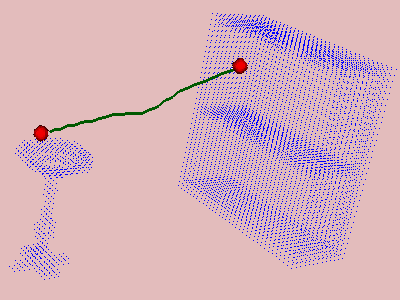
\includegraphics[height=100pt]{figures/Workspace_Path_Barret_1_PinkBG.png} 	
  }
  \subfigure[Execution]{
    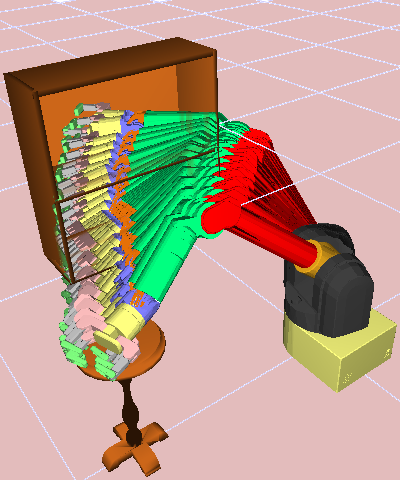
\includegraphics[height=100pt]{figures/Barret_1_Mosaic_small_PinkBG.png} 
  } 
  \caption{ Experiment with a 7-DOF Barret Arm}
  \label{fig:CoverFigure}
\end{figure}


% ***********************************************************
\section{Background}
\label{sec:Background}
The forward kinematics of a manipulator is given as follows:

\begin{equation}
x = f(\q)
\label{eq:FK}
\end{equation}

and its differential version:

\begin{equation}
\dot{x} = \J \dq
\label{eq:Diff_FK}
\end{equation}

where $x \in R^{m}$ and $\q \in R^{n}$, being $m$ and $n$ the dimensions
of the task and joint space respectively. If $m < n$, the manipulator is
task redundant. 

There are two main common manipulator tasks (as described in \cite{seereeram-ns-1995}):

\begin{itemize}
\item{\textit{End-Point Goal:} The manipulator is given start and end task space points. 
The task is to find a sequence of joint space configurations that connect them. 
This is most known as a \textit{path planning problem} } 
\item{\textit{Point-to-Point:} The manipulator is given a task space trajectory to be mapped
to a joint space trajectory. This is most known as a \textit{tracking problem}, which will be 
the focus of this paper.}
\end{itemize}

A particular solution to \ref{eq:Diff_FK}) can be given as:

\begin{equation}
\dq = \Jps \dx
\label{eq:IK_ParticularSol}
\end{equation}

where $\Jps$ is a generalized inverse that can be chosen to minimize a specific criterion. 
In \cite{Whitney-motionRate-1969} Whitney used the Moore-Penrose to minimize the norm of $\dq$. 
Whitney further proposed to use a pseudo-inverse Jacobian weighted with the inertia matrix in 
order to minimize the kinematic energy of the system. A generalization of this is the weighted 
least-norm (WLM) presented in \cite{chan-ns-1995}, which proved to be particularly effective 
to avoid joint limits. Recent extensions to this approach include the work of Xiang with GWLM 
\cite{xiang-ns-2010}.  

The general solution to (\ref{eq:Diff_FK}) can be expressed as:
\begin{equation}
\dq = \Jps \dx + (I - \Jps \J)\dq_{0}
\label{eq:IK_GeneralSol}
\end{equation}
. The second term represents the homogeneous solutions or \textit{self-motions}, that is, motions 
in the configuration space that do not produce motions the task space. 

Homogeneous solutions are configurations in the Jacobian nullspace. These can be found by projecting 
an arbitrary vector $\dq_{0}$ on the nullspace, such as in (\ref{eq:IK_GeneralSol}) where the columns 
of $(I - \Jps \J)$ are the basis of the nullspace of $\J$. Most of the proposed methods differ in 
their choosing of $\dq_{0}$. The most widely used method is the \textit{Gradient projection method} 
(GPM) proposed by Liegeois in \cite{liegeois-ns-1977}. The GPM method consists on defining a 
optimization function $H(\q)$ to be minimized. By defining:

\begin{equation}
\dq_{0} = -\alpha \dfrac{\partial H}{\partial \q}
\end{equation}

it produces solutions that move the manipulator away from undesirable configurations. 
Diverse $H$ functions have been used in the literature, such as the measure manipulatability
 in \cite{yoshikawa-ns-1985}, used to avoid singularities. Other applications include obstacle
avoidance \cite{klein-ns-1985}, minimization of torques \cite{hollerbach-ns-1985}, avoidance
of joint limits \cite{liegeois-ns-1977}, among others. An excellent overview of these early
methods can be found in \cite{siciliano-ns-1990}. For problems with more than one subtask,
nested approaches have been proposed \cite{chiaverini-ns-1997}\cite{nakamura-ns-1987}, 
based on the relative priority between each subtask. Other methods instead define a weigthed
sum of optimization functions, such as in \cite{buss-ns-2006}. 

There are other approaches that tackle the redundancy problem by defining additional constraints
 such that the problem is no longer redundant. Examples of these are the Extended Jacobian 
\cite{baillieul-ns-1985} and the Augmented Jacobian \cite{sciavicco-ns-1988}\cite{egeland-ns-1987}. 

The methods mentioned above solve different kind of problems, however all of them share the same 
weakness of being local, which precludes them to fall in local minima. There are a few global 
approaches such as  but these are rarely used in practice due to the intensive computation required
(Add citations). In the next section we propose a method that attempts to escape the local minima by 
using backtracking in the discretized nullspace of the manipulator.

% *********************************************************
\section{Proposed Algorithm}
\label{sec:ProposedAlgorithm}

We saw in section \ref{sec:Background} that the solution to (\ref{eq:Diff_FK}) has the general form:

\begin{equation}
\dq = \Jps \dx + (I - \Jps \J)\dq_{0}
\label{eq:IK_GeneralSol_2}
\end{equation}

where the second right-hand term represents the self-motions in the Jacobian nullspace, which is a
subspace of dimensions $(n-m)$. Hence, we can write Eq.(\ref{eq:IK_GeneralSol_2}) equivalently as:

\begin{equation}
\dq = \Jps \dx + \displaystyle \sum_{i=1}^{n-m} \nsc_{i}\nsb_{i}
\label{eq:Proposed_Eq1}
\end{equation}

where:
\begin{itemize}
\item{ $\nsb_{i}$: Normalized basis of the Jacobian nullspace}
\item{$\nsc_{i}$: Coefficients of each $\nsb_{i}$}
\end{itemize}

Both representations are equivalent, however (\ref{eq:Proposed_Eq1}) is of special interest to us since
instead of having to define a vector $\q_{0} \in R^{n}$, we define the homogeneous solution in terms of 
the $(n-m)$ coefficient $\nsc_{i}$. The problem, however still has potentially infinite solutions.

Our approach proposes, instead of finding a $\q_{0}$ vector (as GPM does), to effectuate a 
search in the discretized Jacobian nullspace. The discretization is carried out by selecting a range of
values for each $\nsc_{i}$. Notice that, since we are considering the tracking of a task space \textit{trajectory}, 
we do only consider homogeneous solutions that are realizable in one time step. To make this clear, please refer 
to Fig.\ref{fig:SelfMotion_Illustration}. Figures \ref{fig:SelfMotion_Illustration}.a and 
\ref{fig:SelfMotion_Illustration}.c show the one-step self-motions considered. Figures \ref{fig:SelfMotion_Illustration}.b 
and \ref{fig:SelfMotion_Illustration}.d show a subset of the possible self-motions corresponding to these 
that would require more than one time-step to be executed, hence they are not considered in 
the nullspace search explained in this paper\footnote{Notice that in the
general case of tracking a \textit{path}, \textit{all} the self-motion configurations should also be considered. We
are currently working on this topic}.     

% ...............................................
% Self-motion limitation
\begin{figure}[]
  \centering
  \subfigure[One-step self-motion A]{
    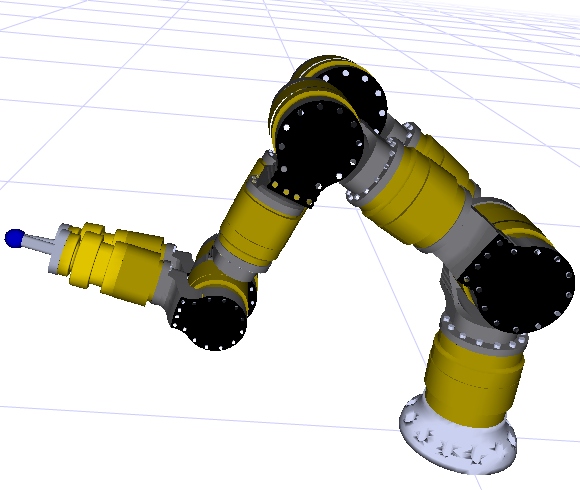
\includegraphics[height=90pt]{figures/singleNS_illustration1.png} }
  \subfigure[Set of self-motions A]{
    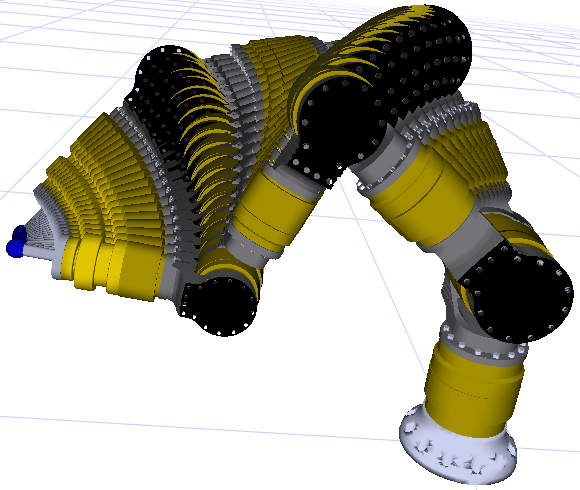
\includegraphics[height=90pt]{figures/completeNS_illustration1.png}
  } \\
  \subfigure[One-step self-motion B]{
    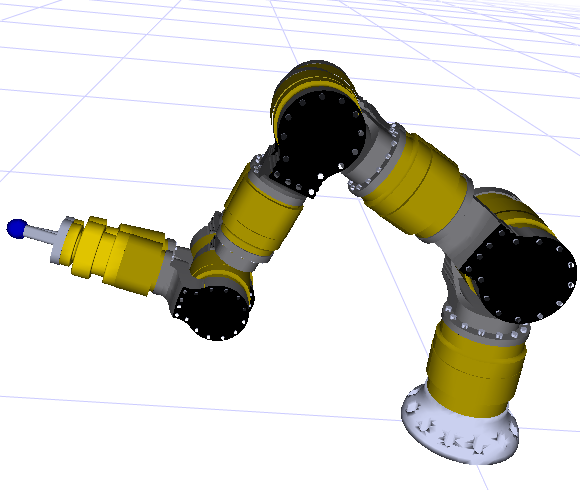
\includegraphics[height=90pt]{figures/singleNS_illustration2.png} 	
  }
  \subfigure[Set of self-motions B]{
    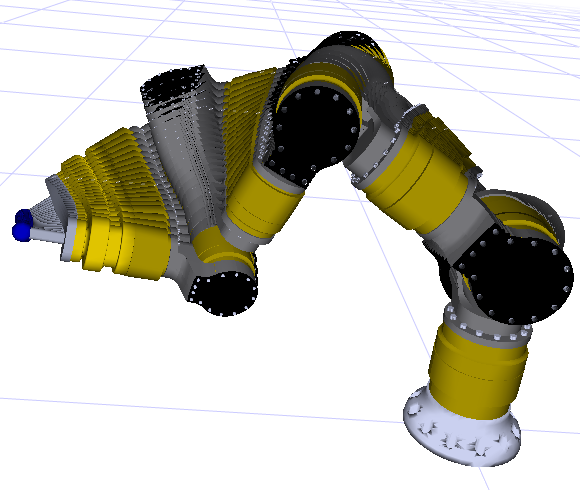
\includegraphics[height=90pt]{figures/completeNS_illustration2.png}
  }  
  \caption{ Illustration of self-motion considered}
  \label{fig:SelfMotion_Illustration}
\end{figure}

Once the set of self-motions is generated we proceed to eliminate the configurations that are in collision, keeping only
the set of \textit{valid} configurations, from which any can be a possible solution for the task space point evaluated.
Rather than picking a random configuration from the nullspace set, we choose a configuration such that it maximizes a
performance optimization function. Previous work such as \cite{kapoor-ns-1998} suggests a serie of diverse functions to assess
the desirability of each configuration. In particular, we have evaluated the so-called Joint Range Availability measurement (JRA):

\begin{equation}
\psi(\q)=  \displaystyle \sum_{i=1}^{n} \dfrac{ \q_{i} - {\bar{\q}}_{i} }{ {\q_{i}}_{Max} - {\q_{i}}_{Min} }
\end{equation}

in our experiments. We save the nullspace sets as priority queues ordered w.r.t. the JRA measure of each configuration. A sketch
of the algorithm explained so far is shown in Algorithm \ref{alg:NaiveSearch}

% -------------------------------------------------------
% FindSequencePaths Algorithm
\begin{algorithm}
%\dontprintsemicolon
\KwIn{ ws \tcp*{workspace path}, q \tcp*{initial configuration} } % \tcp*{problem description}
\KwOut{ wq \tcp*{Jointspace path }  } 
\BlankLine
\SetKwFunction{GenerateNS}{GenerateNS()}
\SetKwFunction{PushQueue}{PushQueue}
\SetKwFunction{EvaluateMeasure}{EvaluateMeasure}
\BlankLine

\For{$i \leftarrow 1$ \KwTo ws.\FuncSty{size()}}{
	\GenerateNS \;

}
\Return a \;
\caption{ NaiveSearch }
\label{alg:NaiveSearch}
\end{algorithm}

So far, our algorithm is completely local, hence it is prone to fall in local minima. We attempt to 





% *********************************************************
\section{Experiments and Results}
\label{sec:Experiments}


% *********************************************************
\section{Conclusions and Future Work}
\label{sec:Conclusions}


% *********************************************************
\section*{Acknowledgments}
The authors would like to thank all members of the Humanoid Lab
at Georgia Tech for their insightful feedback.

% *********************************************************
%\IEEEtriggeratref{8}
%\IEEEtriggercmd{\enlargethispage{-5in}}
\bibliographystyle{IEEEtran}
\bibliography{JnsReferences}


\end{document}


